% Chapter Template

\chapter{Despliegue en Windows} % Main chapter title

\label{Chapter6} % Change X to a consecutive number; for referencing this chapter elsewhere, use \ref{ChapterX}

%----------------------------------------------------------------------------------------
%	SECTION 1
%-------------------------------------------------------------------------------
Para realizar el despliegue sobre las maquinas con sistema operativo Windows se necesitan dos herramientas básicas, adicional a el disco que contiene la imagen base de los nodos de trabajo.

Estas herramientas, son el gestos de máquinas virtuales \textbf{VirtualBox} y el aplicativo que ejecuta los nodos como servicios \textbf{VBoxVMService}.

Estas herramientas se pueden descargar de los enlaces en la Wiki del laboratorio de computación de alto desempeño de la Universidad Tecnológica de Bolívar o ingresando en el navegador la siguiente dirección dentro del campus:

\textit{http://172.16.9.80/ubuntu/spider/workers/}


\section{Pasos para el despliegue en Windows}

\subsection{Instalación de VirtualBox}
Es recomendado que se use la versión 5.0.18 de VirtualBox ya que es la actual al momento de realizar las pruebas. Pueden encontrar el instalador en el enlace de la Wiki.

Se des-instala cualquier versión anterior de VirtualBox y se realiza una instalación fresca de la versión 5.0.18, como administrador.

Una vez finalizada la instalación se procede a crear la máquina que sera el nodo de trabajo.

\subsection{Nodo de trabajo}

\subsubsection*{Creación máquina virtual}
Primero crearemos una máquina virtual con los parámetros de configuración óptimos de acuerdo a la máquina anfitrión (máquina Windows).

La creación de esta maquina es similar a la creación de la máquina base, ver el capitulo 4 de este mismo documento, el cambio esta al usar el Disco Virtual de la máquina base descargada del enlace de la wiki.

Movemos la imagen del disco virtual a la ruta: 

\begin{lstlisting}
C:\Users\"usuario"\VirtualBox VMs
\end{lstlisting}
Donde "usuario" sera remplazado por el nombre del usuario de la máquina windows, y descomprimimos allí nuestra imagen.

Luego al seleccionar la opción ‘‘usar disco virtual existente’’ y colocamos la ruta a nuestro disco virtual base y le damos ‘‘crea’’.

\begin{figure}[h]
\centering
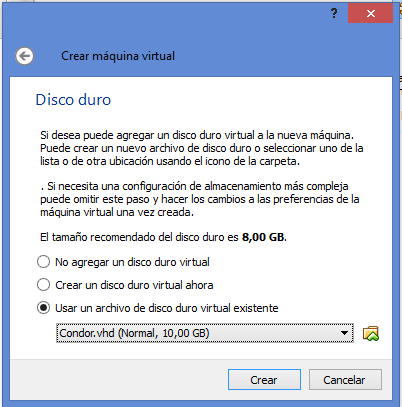
\includegraphics[width=0.8\textwidth]{windows/ddexistente.PNG}
\decoRule
\caption{Disco Virtual Base }
\label{fig:VHD Base}
\end{figure}
\FloatBarrier

Nuestra máquina es creada y procedemos a editar la configuración de esta.

\subsubsection*{Configuración máquina virtual}

Acedemos a la configuración mediante el icono del engranaje en VirtualBox.
Accedemos a la pestaña de sistema donde configuraremos la cantidad de memoria RAM a utilizar y el numero de procesadores.

Es recomendado utilizar el 25\%  de la cantidad total de RAM y el 50\% de los procesadores físicos (1 o 2 máximo).

\begin{figure}[h]
\centering
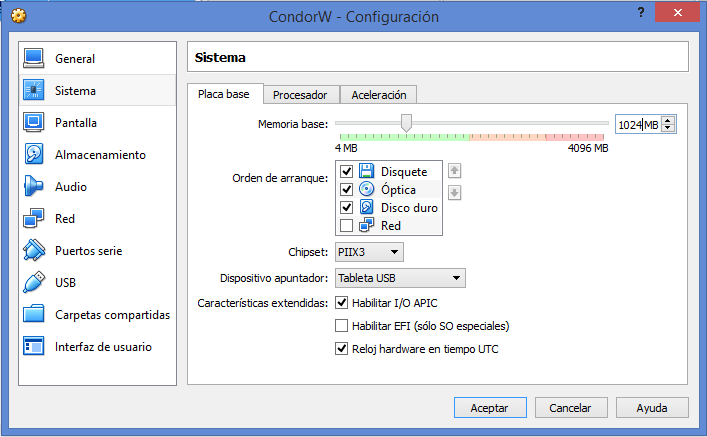
\includegraphics[width=0.8\textwidth]{windows/25ram.PNG}
\decoRule
\caption{Opciones de RAM y procesadores }
\label{fig:VM RAM}
\end{figure}
\FloatBarrier

Luego vamos a la pestaña de Red y colocamos el adaptador de red en modo puente (Bridge Mode), damos aceptar y la maquina esta lista para su primera ejecución.

\begin{figure}[h]
\centering
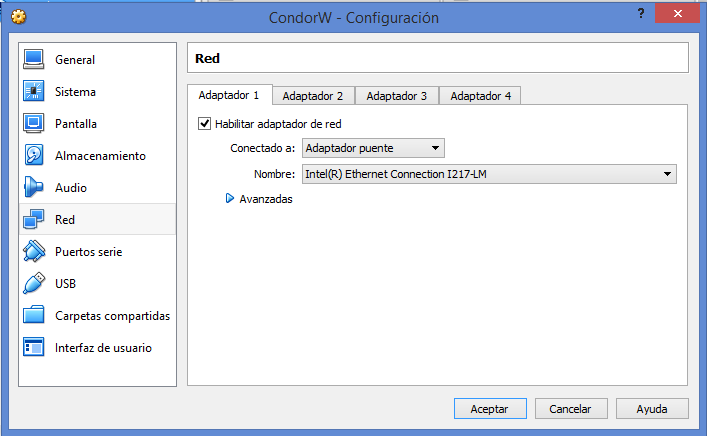
\includegraphics[width=0.8\textwidth]{windows/redpuente.PNG}
\decoRule
\caption{Red Adaptador Puente }
\label{fig:VM NET}
\end{figure}
\FloatBarrier

Ejecutamos la máquina y esperamos que termine la primera ejecución, puede ser algo demorado ya que se reinicia luego de cambiar su nombre.

\begin{figure}[h]
\centering
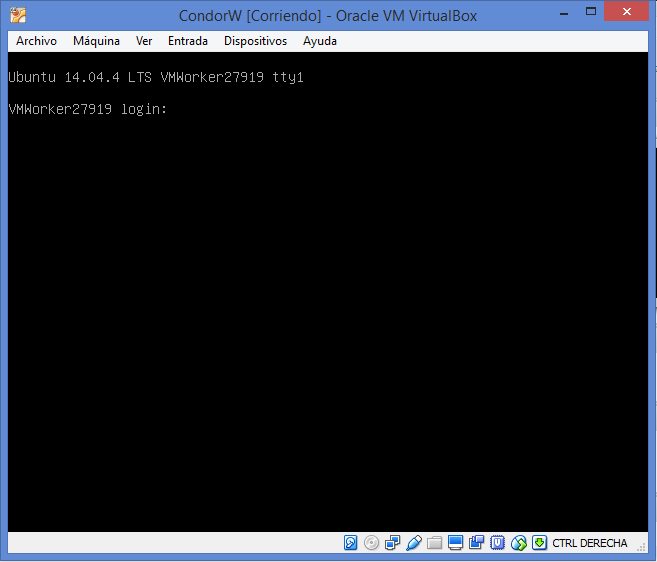
\includegraphics[width=0.9\textwidth]{windows/running.PNG}
\decoRule
\caption{Máquina virtual en funcionamiento}
\label{fig:VM Running}
\end{figure}
\FloatBarrier

Ahora se procede a configurar la máquina para ejecución en segundo plano, como servicio.

\subsubsection*{Máquina Virtual como servicio}

Para ejecutar la máquina virtual en background (no se creará ni se ejecutará la consola de administración de VirtualBox, ni la consola de ejecución de la máquina virtual) se instala la herramienta VBoxVMService.

Se cierra por completo VirtualBox y ejecutamos como administrador el instalador de VBoxVMService.
Se procede con la instalación sin cambiar la ubicación de instalación, una vez completada la instalación, finalizamos y vamos a la carpeta conde fue instalado.

\begin{lstlisting}
C:\vms
\end{lstlisting}

Allí se modifica el archivo \textbf{\textit{VBoxVmService}} que es el archivo de configuración.

\begin{figure}[h]
\centering
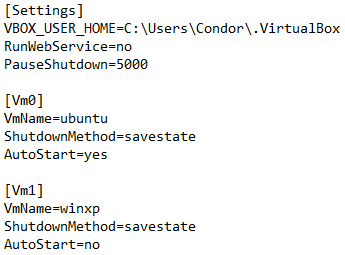
\includegraphics[width=0.75\textwidth]{windows/vmservice.PNG}
\decoRule
\caption{Archivo de configuración}
\label{fig:vms config}
\end{figure}
\FloatBarrier

Editamos los parámetros para que nuestra máquina virtual \textbf{\textit{CondorW}} inicie como servicio, y el método de apagado sea total, no guarde el estado en que se encontraba.

\begin{figure}[h]
\centering
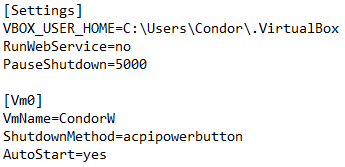
\includegraphics[width=0.75\textwidth]{windows/condorw.PNG}
\decoRule
\caption{Configuración final CondorW}
\label{fig:vms final}
\end{figure}
\FloatBarrier

Reiniciamos nuestra máquina anfitrión y nos aseguramos que al iniciar nuevamente nuestro nodo de trabajo se esta ejecutando en background.

\begin{figure}[h]
\centering
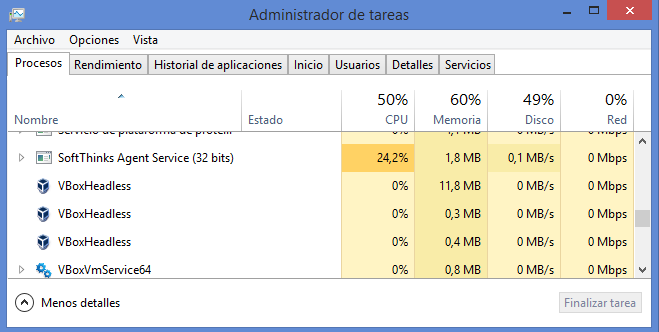
\includegraphics[width=0.75\textwidth]{windows/tasks.PNG}
\decoRule
\caption{Procesos en segundo plano en Windows}
\label{fig:task manager}
\end{figure}
\FloatBarrier

Se puede apreciar que esta en ejecución VBoxVmService y tres procesos Headless que son los que indican que nuestra maquina esta en ejecución en background.







%---------------------------------------------------------------------------